\documentclass[11pt,a4paper]{article}
\usepackage[a4paper,margin=24mm,top=22mm,bottom=22mm]{geometry}
\usepackage[T1]{fontenc}
\usepackage{newpxtext,newpxmath}
\usepackage{microtype}
\usepackage{amsmath,mathtools}
\usepackage{tikz}
\usetikzlibrary{arrows.meta,calc,positioning}
\usepackage[most]{tcolorbox}
\usepackage{enumitem}
\usepackage{needspace}
\usepackage{fancyhdr}
\usepackage{titlesec}
\usepackage{array,booktabs}
\usepackage{xcolor}
\usepackage{hyperref}
\definecolor{ink}{HTML}{15253B}
\definecolor{blue}{HTML}{1B567B}
\definecolor{muted}{HTML}{586779}
\definecolor{pale}{HTML}{F1F6FA}
\definecolor{line}{HTML}{C8D9E6}
\definecolor{warm}{HTML}{FFF8E9}
\definecolor{gold}{HTML}{AA792C}
\hypersetup{colorlinks=true,linkcolor=blue,urlcolor=blue,pdftitle={From a random walk to the heat equation: a slow derivation},pdfauthor={Undergraduate guided notes}}
\setlength{\parindent}{0pt}
\setlength{\parskip}{6pt}
\setlength{\emergencystretch}{2em}
\linespread{1.06}
\pagestyle{fancy}
\fancyhf{}
\fancyhead[L]{\footnotesize\color{muted} RANDOM WALK $\longrightarrow$ HEAT EQUATION}
\fancyhead[R]{\footnotesize\color{muted} GUIDED DERIVATION}
\fancyfoot[C]{\footnotesize\color{muted}\thepage}
\renewcommand{\headrulewidth}{0pt}
\titleformat{\section}{\Large\bfseries\color{ink}}{}{0pt}{}
\titleformat{\subsection}{\normalsize\bfseries\color{blue}}{}{0pt}{}
\titlespacing*{\section}{0pt}{20pt}{7pt}
\titlespacing*{\subsection}{0pt}{14pt}{4pt}
\newtcolorbox{think}[1][]{enhanced,breakable,colback=warm,colframe=gold!45!white,boxrule=.6pt,arc=1.5mm,left=3.5mm,right=3.5mm,top=2.5mm,bottom=2mm,before skip=11pt,after skip=11pt,title={\bfseries\small STOP AND THINK},coltitle=gold,fonttitle=\sffamily,#1}
\newtcolorbox{takeaway}[1][]{enhanced,breakable,colback=pale,colframe=line,boxrule=.7pt,arc=1.5mm,left=4mm,right=4mm,top=3mm,bottom=3mm,before skip=12pt,after skip=12pt,#1}
\newcommand{\ans}[1]{\par\vspace{4pt}{\small\color{blue}\textbf{Answer.}}\enspace #1}
\newcommand{\dd}{\Delta}
\newcommand{\jp}{p_j^{\,n}}
\newcommand{\jum}{p_{j-1}^{\,n}}
\newcommand{\jup}{p_{j+1}^{\,n}}
\newcommand{\jnext}{p_j^{\,n+1}}
\newcommand{\spacebar}{\hspace{0.3em}}
\newcommand{\aside}[1]{{\small\color{muted}#1}}
\begin{document}
\begin{center}
{\fontsize{23}{27}\selectfont\bfseries\color{ink} From a Random Walk\\[3pt]to the Heat Equation}\par
\vspace{8pt}
{\large\color{blue} A patient derivation, one small step at a time}\par
\vspace{9pt}
{\small\color{muted} One particle. Two possible jumps. One equation for how probabilities spread.}
\end{center}
\vspace{3pt}
\begin{takeaway}
\textbf{The destination.}\quad We want to understand how the very simple rule
\begin{center}
\emph{``Move one place left or one place right, each with probability $\tfrac12$''}
\end{center}
leads, when distances and time steps are sufficiently small, to
\[
\boxed{\displaystyle \frac{\partial u}{\partial t}=D\frac{\partial^2u}{\partial x^2}.}
\]
We will not assume this equation or even its meaning. We will build it from the walking rule. The important part is \emph{why the discrete description can become a continuous one}.
\end{takeaway}

\section{1. First picture: one particle on a line}
Imagine a row of equally spaced positions, labelled
\[
\ldots,-3,-2,-1,0,1,2,3,\ldots.
\]
A particle begins at position $0$. Every time a bell rings, it makes exactly \emph{one} jump. It cannot remain where it is.
\begin{itemize}[leftmargin=20pt,itemsep=2pt,topsep=2pt]
\item With probability $\tfrac12$, it moves one place \textbf{left}.
\item With probability $\tfrac12$, it moves one place \textbf{right}.
\end{itemize}
Its next jump is independent of its earlier jumps: each time, it makes a fresh left-or-right choice.

\begin{center}
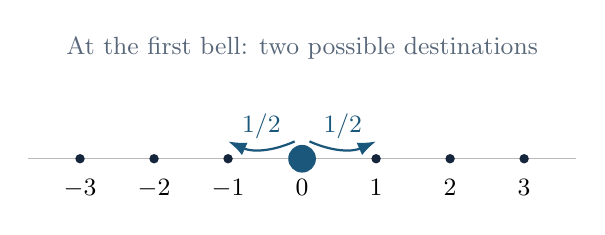
\begin{tikzpicture}[x=.94cm,y=1cm,>=Latex]
\draw[gray!55,thin] (-3.7,0)--(3.7,0);
\foreach \j in {-3,...,3}{\fill[ink] (\j,0) circle (1.7pt);\node[below=4pt,font=\small] at (\j,0) {$\j$};}
\fill[blue] (0,0) circle (5pt);
\draw[->,thick,blue] (-.1,.22) to[bend left=24] node[above,font=\small] {$1/2$} (-1,.22);
\draw[->,thick,blue] (.1,.22) to[bend right=24] node[above,font=\small] {$1/2$} (1,.22);
\node[above=14pt,font=\small\color{muted}] at (0,.65) {At the first bell: two possible destinations};
\end{tikzpicture}
\end{center}

\begin{think}
Can the particle be at position $0$ after \emph{one} jump? Can it be at position $0$ after \emph{two} jumps?
\ans{After one jump, no: it must be at $-1$ or $1$. After two jumps, yes: left then right, or right then left, returns it to $0$.}
\end{think}

\section{2. The question we really want to ask}
The position of any particular particle is unpredictable. So instead of asking, ``Where \emph{will} it be?'', ask:
\begin{center}
\emph{``What is the probability that it is at a particular position, after a particular number of jumps?''}
\end{center}
Introduce notation very deliberately:
\[
\boxed{p_j^{\,n}=\text{probability of being at position $j$ after $n$ jumps}.}
\]
The lower label $j$ tells us \emph{where}; the upper label $n$ tells us \emph{when}. Neither label is a power.

For example, $p_0^{\,0}=1$: at the start, the particle is certainly at $0$. Also $p_1^{\,0}=0$: at the start, it is certainly \emph{not} at $1$.

\begin{think}
What are $p_{-1}^{\,1}$, $p_0^{\,1}$ and $p_1^{\,1}$?
\ans{$p_{-1}^{\,1}=\tfrac12$, $p_0^{\,1}=0$ and $p_1^{\,1}=\tfrac12$. There are only two places the first jump can reach.}
\end{think}

\newpage
\section{3. Follow the walk for just two jumps}
Before writing a general formula, calculate one probability directly. We want $p_0^{\,2}$: the probability of returning to $0$ after two jumps.

There are exactly two routes that return to $0$:
\begin{center}
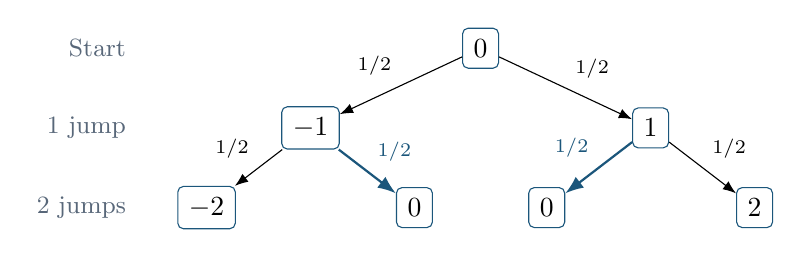
\begin{tikzpicture}[x=1.2cm,y=.92cm,>=Latex]
\node[draw=blue,rounded corners=2pt,inner sep=4pt] (o) at (0,0) {$0$};
\node[draw=blue,rounded corners=2pt,inner sep=4pt] (l) at (-1.8,-1.1) {$-1$};
\node[draw=blue,rounded corners=2pt,inner sep=4pt] (r) at (1.8,-1.1) {$1$};
\node[draw=blue,rounded corners=2pt,inner sep=4pt] (ll) at (-2.9,-2.2) {$-2$};
\node[draw=blue,rounded corners=2pt,inner sep=4pt] (lr) at (-.7,-2.2) {$0$};
\node[draw=blue,rounded corners=2pt,inner sep=4pt] (rl) at (.7,-2.2) {$0$};
\node[draw=blue,rounded corners=2pt,inner sep=4pt] (rr) at (2.9,-2.2) {$2$};
\draw[->,thin] (o)--node[above left,font=\scriptsize] {$1/2$}(l);
\draw[->,thin] (o)--node[above right,font=\scriptsize] {$1/2$}(r);
\draw[->,thin] (l)--node[above left,font=\scriptsize] {$1/2$}(ll);
\draw[->,thick,blue] (l)--node[above right,font=\scriptsize] {$1/2$}(lr);
\draw[->,thick,blue] (r)--node[above left,font=\scriptsize] {$1/2$}(rl);
\draw[->,thin] (r)--node[above right,font=\scriptsize] {$1/2$}(rr);
\node[left,font=\small\color{muted}] at (-3.65,0) {Start};
\node[left,font=\small\color{muted}] at (-3.65,-1.1) {1 jump};
\node[left,font=\small\color{muted}] at (-3.65,-2.2) {2 jumps};
\end{tikzpicture}
\end{center}

The route \emph{left, then right} has probability
\[
\frac12\times\frac12=\frac14.
\]
The route \emph{right, then left} also has probability $\tfrac14$. Since either route will do, we \emph{add} their probabilities:
\[
\boxed{p_0^{\,2}=\frac14+\frac14=\frac12.}
\]
The remaining probability is divided equally between $-2$ and $2$.

\begin{center}
\begin{tabular}{@{}c|ccccc@{}}
\toprule
Position $j$ & $-2$ & $-1$ & $0$ & $1$ & $2$\\
\midrule
Probability after 2 jumps, $p_j^{\,2}$ & $\frac14$ & $0$ & $\frac12$ & $0$ & $\frac14$\\
\bottomrule
\end{tabular}
\end{center}

\begin{think}
Why do we \emph{multiply} probabilities along a route, but \emph{add} probabilities for two different routes?
\ans{To follow one particular route, both independent choices must happen. To reach $0$, either of two mutually exclusive routes can happen.}
\end{think}

\clearpage
\section{4. A general rule: how can we arrive at $j$?}
Now choose \emph{any} position $j$, and imagine the particle arriving there on the next jump.

\textbf{Where could it have been immediately before that jump?} Only at the neighbouring positions:
\begin{itemize}[leftmargin=20pt,itemsep=3pt,topsep=2pt]
\item At $j-1$, followed by a jump \emph{right}.
\item At $j+1$, followed by a jump \emph{left}.
\end{itemize}
There is no third possibility: the particle always moves exactly one place.

\begin{center}
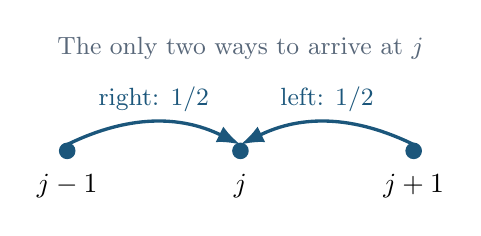
\begin{tikzpicture}[x=2.2cm,y=1cm,>=Latex]
\foreach \x/\txt in {-1/{j-1},0/j,1/{j+1}} {
 \fill[blue] (\x,0) circle (3pt);
 \node[below=5pt,font=\normalsize] at (\x,0) {$\txt$};
}
\draw[->,very thick,blue] (-1,.08) to[bend left=26] node[above,font=\small] {right: $1/2$} (0,.08);
\draw[->,very thick,blue] (1,.08) to[bend right=26] node[above,font=\small] {left: $1/2$} (0,.08);
\node[above=14pt,font=\small\color{muted}] at (0,.55) {The only two ways to arrive at $j$};
\end{tikzpicture}
\end{center}

\subsection*{Now derive the discrete equation, one route at a time}
Let us calculate the contribution from each route, one line at a time.

\textbf{Route A: from $j-1$ to $j$.}\\
The chance that the particle is at $j-1$ after $n$ jumps is $p_{j-1}^{\,n}$. Given that it is there, the chance of jumping right is $\tfrac12$. Hence
\[
\underbrace{\Pr(\text{route A})}_{\text{arrive from the left}}
=\underbrace{p_{j-1}^{\,n}}_{\text{at $j-1$ after $n$ jumps}}
\times\underbrace{\frac12}_{\text{jump right}}
=\frac12p_{j-1}^{\,n}.
\]

\textbf{Route B: from $j+1$ to $j$.}\\
By exactly the same reasoning,
\[
\underbrace{\Pr(\text{route B})}_{\text{arrive from the right}}
=\underbrace{p_{j+1}^{\,n}}_{\text{at $j+1$ after $n$ jumps}}
\times\underbrace{\frac12}_{\text{jump left}}
=\frac12p_{j+1}^{\,n}.
\]

These two routes cannot occur simultaneously on the same jump. And they exhaust all the ways of reaching $j$. Therefore we \emph{add}:
\[
\boxed{\displaystyle p_j^{\,n+1}=\frac12p_{j-1}^{\,n}+\frac12p_{j+1}^{\,n}.}
\tag{1}
\]
\begin{takeaway}
\textbf{Read equation (1) in words.} The probability of being at $j$ \emph{one jump later} equals half the previous probability at the left neighbour, plus half the previous probability at the right neighbour.

This is the \textbf{discrete evolution equation}. It follows \emph{exactly} from the rules of the walk. No approximation has been made.
\end{takeaway}

\begin{think}
Check (1) when $j=0$ and $n=1$. Does it reproduce our earlier answer for $p_0^{\,2}$?
\ans{Yes. $p_0^{\,2}=\tfrac12p_{-1}^{\,1}+\tfrac12p_1^{\,1}=\tfrac12\cdot\tfrac12+\tfrac12\cdot\tfrac12=\tfrac12$.}
\end{think}

\section{5. Pause: what is this equation saying?}
Suppose the probability at a position is greater than at either neighbour. On the next step it becomes the \emph{average of the neighbouring probabilities}, so it tends to decrease. If the probability at a position is lower than those around it, it tends to increase.

That is the first sign of \emph{spreading}. We have not mentioned heat yet; nevertheless, the mathematics already describes a quantity redistributing itself from relatively high values towards relatively low ones.

\aside{There is one subtlety: for a particle starting at a single grid point, the probabilities initially occupy alternating sites. We will use a smooth description only at scales where this microscopic pattern has been averaged out. The appendix explains this carefully.}

\section{6. What would it mean to make the walk continuous?}
So far, position comes in whole numbers ($\ldots,-1,0,1,\ldots$) and time is counted in whole jumps ($0,1,2,\ldots$). But the heat equation describes a quantity at \emph{any} position $x$ and \emph{any} time $t$.

We cannot simply replace the letters $j$ and $n$ by $x$ and $t$. We must say what happens to the spacing between the allowed positions and to the time between jumps.

Let
\[
\begin{aligned}
 h&=\text{physical distance of one jump},\\
 \tau&=\text{physical time between jumps}.
\end{aligned}
\]
Then the grid point labelled $j$ has physical position $x=jh$. The instant after $n$ jumps is $t=n\tau$.

\begin{center}
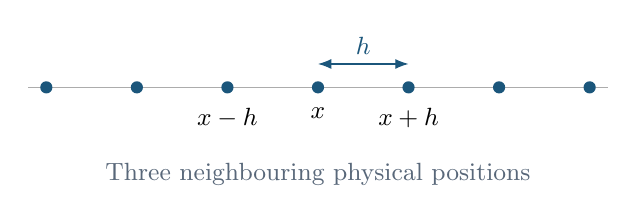
\begin{tikzpicture}[x=1.15cm,y=.9cm,>=Latex]
\draw[gray!65] (-3.2,0)--(3.2,0);
\foreach \i in {-3,...,3}{\fill[blue] (\i,0) circle (2.2pt);}
\draw[<->,blue] (0,.33)--node[above,font=\small] {$h$}(1,.33);
\node[below=4pt,font=\small] at (-1,0) {$x-h$};
\node[below=4pt,font=\small] at (0,0) {$x$};
\node[below=4pt,font=\small] at (1,0) {$x+h$};
\node[below=24pt,font=\small\color{muted}] at (0,0) {Three neighbouring physical positions};
\end{tikzpicture}
\end{center}

\textbf{The idea of a continuous approximation.} Imagine describing the distribution on a scale much wider than the individual jumps. Instead of looking at every tiny up-and-down of the grid values, imagine a smooth profile $u(x,t)$ that represents their overall shape.

For now, think of $u$ simply as the \emph{height of that smooth profile}. Its numerical scale is unimportant: the same fixed conversion factor is used for every site, and that factor will cancel out of our equation.

\begin{takeaway}[unbreakable]
We make one \textbf{new assumption}: at the scale we want to describe, a sufficiently smoothed version of the probabilities changes gradually from one nearby position to the next, and gradually over one short time step.

This is an \emph{assumption about the large-scale description}; it is not a claim that the raw probabilities are already smooth at every step.
\end{takeaway}

\begin{think}
If $h$ is small, what are the physical positions immediately to the left and right of $x$? If $\tau$ is small, when is the next jump after time $t$?
\ans{The neighbours are at $x-h$ and $x+h$. The next jump occurs at time $t+\tau$.}
\end{think}

\section{7. Translate the discrete rule without changing it}
Recall our exact equation:
\[
 p_j^{\,n+1}=\frac12p_{j-1}^{\,n}+\frac12p_{j+1}^{\,n}.
\]
Read it again in physical coordinates:
\begin{itemize}[leftmargin=21pt,itemsep=4pt]
\item $j$ means position $x$.
\item $j-1$ means position $x-h$.
\item $j+1$ means position $x+h$.
\item $n$ means time $t$; $n+1$ means time $t+\tau$.
\end{itemize}
If the smoothed probability profile is represented by $u$, the \emph{same update pattern} becomes
\[
\boxed{u(x,t+\tau)\ \approx\ \frac12u(x-h,t)+\frac12u(x+h,t).}
\tag{2}
\]
The $\approx$ sign matters: equation (1) was exact for grid probabilities; equation (2) is our smooth, large-scale approximation.

\newpage
\section{8. First rearrangement: isolate the change in time}
To find an equation describing how $u$ changes, subtract $u(x,t)$ from both sides of (2):
\[
\begin{aligned}
 u(x,t+\tau)-u(x,t)
 &\approx \tfrac12u(x-h,t)+\tfrac12u(x+h,t)-u(x,t).
\end{aligned}
\]
Why is that useful? Because the left-hand side is now precisely
\[
\underbrace{u(x,t+\tau)-u(x,t)}_{\text{new height $-$ old height at the same position}}.
\]
This is a change in height during one time step.

Rewrite the right-hand side so it has just one fraction:
\[
\boxed{\displaystyle
u(x,t+\tau)-u(x,t)
\approx \frac{u(x-h,t)-2u(x,t)+u(x+h,t)}{2}.}
\tag{3}
\]
The $-2u(x,t)$ is not magic: subtracting $u(x,t)$ is the same as subtracting $\tfrac12u(x,t)$ twice.

\begin{think}
Suppose at one instant the three heights (left, centre, right) are $3$, $5$, $4$. What does (2) predict for the centre at the next instant?
\ans{It predicts $\tfrac12(3)+\tfrac12(4)=3.5$. The centre falls from $5$ to $3.5$, a change of $-1.5$. Equation (3) gives $(3-10+4)/2=-1.5$, exactly the same change.}
\end{think}

\section{9. Turn the change into a rate of change}
The difference $u(x,t+\tau)-u(x,t)$ is a \emph{change over one time step}. To find the average \emph{rate} of change, divide by the duration $\tau$:
\[
\frac{u(x,t+\tau)-u(x,t)}{\tau}.
\]
This is the familiar idea \emph{change divided by elapsed time}. If the profile changes smoothly and $\tau$ is very small, that average rate is close to the instantaneous rate:
\[
\underbrace{\frac{u(x,t+\tau)-u(x,t)}{\tau}}_{\text{rate across a short time step}}
\quad\longrightarrow\quad
\underbrace{\frac{\partial u}{\partial t}(x,t)}_{\text{instantaneous rate at fixed $x$}}.
\]
The symbol $\partial/\partial t$ just reminds us to change \emph{time} while keeping the position $x$ fixed.

Divide equation (3) by $\tau$:
\[
\boxed{\displaystyle
\frac{u(x,t+\tau)-u(x,t)}{\tau}
\approx
\frac{u(x-h,t)-2u(x,t)+u(x+h,t)}{2\tau}.}
\tag{4}
\]
We can now see the \textbf{time derivative} emerging on the left of (4). Next we must understand why the particular combination of three heights on the right measures a \textbf{second spatial derivative}.

\newpage
\section{10. Why does a second spatial derivative appear?}
Hold time $t$ fixed. Draw three nearby points on the smooth profile: one at $x-h$, one at $x$, and one at $x+h$.

A \emph{first} derivative measures slope. We can estimate the slope on either side of $x$:
\[
\begin{aligned}
\text{left slope}\quad L&=\frac{u(x,t)-u(x-h,t)}{h},\\[5pt]
\text{right slope}\quad R&=\frac{u(x+h,t)-u(x,t)}{h}.
\end{aligned}
\]
Read these formulas before going on. Each is \emph{change in height divided by horizontal distance}.

\begin{center}
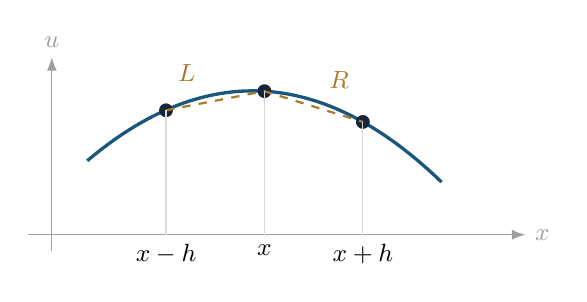
\begin{tikzpicture}[x=1.25cm,y=.85cm,>=Latex]
\draw[->,gray!75] (-2.4,0)--(2.65,0) node[right,font=\small] {$x$};
\draw[->,gray!75] (-2.16,-.25)--(-2.16,2.65) node[above,font=\small] {$u$};
\draw[blue,very thick,domain=-1.8:1.8,smooth,variable=\z,samples=60] plot ({\z},{2.15-.37*(\z+.12)^2});
\coordinate (a) at (-1,1.86);\coordinate (b) at (0,2.145);\coordinate (c) at (1,1.686);
\fill[ink] (a) circle (2.5pt) (b) circle (2.5pt) (c) circle (2.5pt);
\draw[dashed,gold,thick] (a)--(b)--(c);
\node[below,font=\small] at (-1,0) {$x-h$};
\node[below,font=\small] at (0,0) {$x$};
\node[below,font=\small] at (1,0) {$x+h$};
\draw[gray!30] (-1,0)--(a) (0,0)--(b) (1,0)--(c);
\node[above left,font=\small\color{gold}] at (-.6,2.15) {$L$};
\node[above right,font=\small\color{gold}] at (.56,2.04) {$R$};
\end{tikzpicture}
\end{center}

A \emph{second} derivative measures how quickly the \emph{slope itself} is changing. So it is natural to compute \emph{right slope minus left slope}, then divide by the distance $h$:
\[
\begin{aligned}
\frac{R-L}{h}
&=\frac{1}{h}\left(\frac{u(x+h,t)-u(x,t)}{h}
-\frac{u(x,t)-u(x-h,t)}{h}\right)\\[5pt]
&=\boxed{\displaystyle\frac{u(x-h,t)-2u(x,t)+u(x+h,t)}{h^2}.}
\end{aligned}
\]
Nothing has been approximated in this algebra. The expression on the right is the \textbf{difference between two neighbouring slopes, per unit distance}.

For a smooth profile, as $h$ becomes very small, this approaches the second derivative:
\[
\boxed{\displaystyle
\frac{u(x-h,t)-2u(x,t)+u(x+h,t)}{h^2}
\quad\longrightarrow\quad
\frac{\partial^2u}{\partial x^2}(x,t).}
\tag{5}
\]
\begin{think}
At the top of a rounded hill, does the slope become more positive or more negative as we move from left to right?
\ans{More negative: the curve first rises, flattens, then falls. So its second derivative is negative at the top of the hill.}
\end{think}

\newpage
\section{11. Put the two pieces together}
Return to equation (4). It contains a short-time change on the left and the three-point spatial expression on the right:
\[
\frac{u(x,t+\tau)-u(x,t)}{\tau}
\approx
\frac{u(x-h,t)-2u(x,t)+u(x+h,t)}{2\tau}.
\]
We would like to use the spatial expression from (5), which has $h^2$ in the denominator. So multiply and divide the right-hand side by $h^2$:
\[
\boxed{\displaystyle
\frac{u(x,t+\tau)-u(x,t)}{\tau}
\approx
\underbrace{\frac{h^2}{2\tau}}_{\text{one constant}}
\underbrace{\frac{u(x-h,t)-2u(x,t)+u(x+h,t)}{h^2}}_{\text{change of slope per unit distance}}.}
\tag{6}
\]
Pause on this formula. The factor $h^2$ has \emph{not} appeared from nowhere. We deliberately multiplied and divided by the same quantity, so the right-hand side is unchanged.

\subsection*{What happens if the jumps become tiny?}
We now imagine studying finer and finer walks: $h$ becomes small, and $\tau$ also becomes small. But \emph{how} should they shrink relative to each other?

To obtain an interesting, finite equation, we assume
\[
\boxed{\displaystyle \frac{h^2}{2\tau}\longrightarrow D,\qquad 0<D<\infty.}
\tag{7}
\]
Here $D$ is a fixed positive number. Equation (7) says that if we halve the jump distance, we should make the time between jumps \emph{four times shorter}, not merely twice as short.

\begin{center}
\begin{tabular}{@{}ccc@{}}
\toprule
Jump distance $h$ & Time per jump $\tau$ & $h^2/(2\tau)$\\
\midrule
$1$ & $1/2$ & $1$\\
$1/2$ & $1/8$ & $1$\\
$1/4$ & $1/32$ & $1$\\
\bottomrule
\end{tabular}
\end{center}

\begin{think}
If $h$ is divided by $10$, what must happen to $\tau$ to keep $D=h^2/(2\tau)$ unchanged?
\ans{$\tau$ must be divided by $100$, because the square of $1/10$ is $1/100$.}
\end{think}

\textbf{Now take the continuous approximation.} Under the smoothness assumption from Section 6, the left-hand quotient in (6) approaches $u_t$ and the right-hand spatial quotient approaches $u_{xx}$. Under the scaling assumption (7), the coefficient approaches $D$.

Therefore the macroscopic profile obeys
\[
\boxed{\displaystyle \frac{\partial u}{\partial t}=D\frac{\partial^2u}{\partial x^2}.}
\tag{8}
\]
This is the \textbf{one-dimensional heat equation}, also called the \textbf{diffusion equation}.

\newpage
\section{12. Why should this equation describe spreading?}
We have derived (8) symbolically. Let us check whether it agrees with the simple picture of a random walk.

\textbf{At the top of a rounded hill:} the second spatial derivative is negative. Hence
\[
 u_{xx}<0\quad\Longrightarrow\quad u_t=Du_{xx}<0
\]
when $D>0$. So the height of the hill \emph{decreases} as time passes.

\textbf{At the bottom of a rounded valley:} the second spatial derivative is positive. Hence
\[
 u_{xx}>0\quad\Longrightarrow\quad u_t=Du_{xx}>0.
\]
So the valley \emph{fills in} as time passes.

\begin{center}
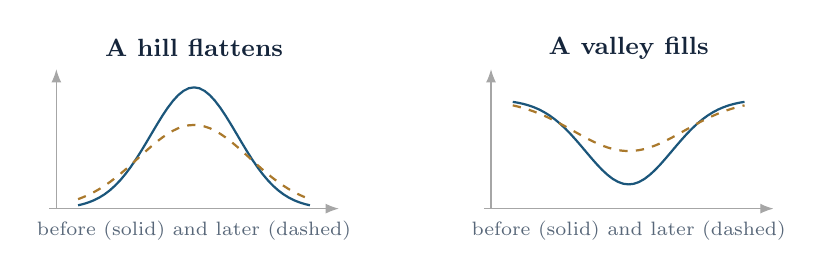
\begin{tikzpicture}[x=.92cm,y=.77cm,>=Latex]
\begin{scope}[shift={(-3.0,0)}]
 \draw[->,gray!70] (-2,0)--(2,0);
 \draw[->,gray!70] (-1.9,0)--(-1.9,2.3);
 \draw[thick,blue,domain=-1.6:1.6,samples=45] plot (\x,{2*exp(-1.4*\x*\x)});
 \draw[thick,dashed,gold,domain=-1.6:1.6,samples=45] plot (\x,{1.38*exp(-.85*\x*\x)});
 \node[font=\small\bfseries\color{ink}] at (0,2.65) {A hill flattens};
 \node[font=\scriptsize\color{muted}] at (0,-.36) {before (solid) and later (dashed)};
\end{scope}
\begin{scope}[shift={(3.0,0)}]
 \draw[->,gray!70] (-2,0)--(2,0);
 \draw[->,gray!70] (-1.9,0)--(-1.9,2.3);
 \draw[thick,blue,domain=-1.6:1.6,samples=45] plot (\x,{1.8-1.4*exp(-1.4*\x*\x)});
 \draw[thick,dashed,gold,domain=-1.6:1.6,samples=45] plot (\x,{1.8-.85*exp(-.85*\x*\x)});
 \node[font=\small\bfseries\color{ink}] at (0,2.65) {A valley fills};
 \node[font=\scriptsize\color{muted}] at (0,-.36) {before (solid) and later (dashed)};
\end{scope}
\end{tikzpicture}
\end{center}

Notice that the equation does \emph{not} say ``movement is always from left to right''. It says that the shape tends to become \emph{less uneven}. That matches a particle whose successive jumps have no preferred direction, yet whose possible positions become increasingly spread out.

\clearpage
\section{13. What assumptions did we actually make?}
It is important to separate what we \emph{proved from the rules of the walk} from what we \emph{assumed to obtain a smooth equation}.

\begin{enumerate}[leftmargin=21pt,itemsep=6pt]
\item \textbf{The particle's rule:} one left or right jump every $\tau$ units of time, each with probability $1/2$; fresh independent choices each time. This gives equation (1) exactly.
\item \textbf{A large-scale, smooth description exists:} when we look beyond the microscopic alternation of occupied sites, the probability profile can be approximated by a function $u(x,t)$ whose nearby heights and slopes vary gradually.
\item \textbf{The steps are small compared with the scales of interest:} both $h$ and $\tau$ are sufficiently small that short difference quotients approximate derivatives.
\item \textbf{Space and time shrink together:} $h^2/(2\tau)$ tends to a fixed, nonzero number $D$. Without that relationship, our limiting equation need not be the heat equation.
\end{enumerate}

\begin{takeaway}
\textbf{The entire argument in four lines:}
\begin{align*}
\text{random walk:}\quad &p_j^{\,n+1}=\tfrac12(p_{j-1}^{\,n}+p_{j+1}^{\,n}),\\[2pt]
\text{smooth description:}\quad &u(x,t+\tau)\approx\tfrac12[u(x-h,t)+u(x+h,t)],\\[2pt]
\text{rearrange:}\quad &\frac{u(x,t+\tau)-u(x,t)}{\tau}\approx\frac{h^2}{2\tau}\frac{u(x-h,t)-2u(x,t)+u(x+h,t)}{h^2},\\[2pt]
\text{small-step limit:}\quad &\boxed{u_t=D u_{xx}.}
\end{align*}
\end{takeaway}

\clearpage
\appendix
\section*{Appendix A. Questions worth returning to}
The derivation above was deliberately guided, rather than a full proof of convergence. These notes address the questions that are easy to miss on a first reading.

\subsection*{A1. Why can we not draw a smooth curve through the exact probabilities straight away?}
After one jump, only the \emph{odd} sites can be occupied. After two jumps, only the \emph{even} sites can be occupied. This alternation continues forever: half the sites have zero probability at each particular step.

So the raw sequence $\ldots,p_{-1}^{\,n},p_0^{\,n},p_1^{\,n},\ldots$ can zigzag between zero and a positive value, even after many jumps. A smooth curve through \emph{all} the raw heights is not justified.

One elementary repair is to average two consecutive time levels:
\[
 q_j^{\,n}=\tfrac12\bigl(p_j^{\,n}+p_j^{\,n+1}\bigr).
\]
This puts weight on both types of sites. Moreover, because the original update is linear, the new $q_j^{\,n}$ satisfies the very same update rule:
\[
 q_j^{\,n+1}=\tfrac12\bigl(q_{j-1}^{\,n}+q_{j+1}^{\,n}\bigr).
\]
After many steps, this averaged profile is the kind of object we may reasonably approximate by a smooth shape. A completely rigorous treatment needs to specify precisely in what sense the profiles approach one another.

\begin{think}
Why is it helpful that averaging does \emph{not} change the form of the update equation?
\ans{We can remove the distracting left-right alternation without having to derive a new kind of evolution law. The same algebra that led to the heat equation still works.}
\end{think}

\subsection*{A2. What does the height $u(x,t)$ really measure?}
At a fixed site, $p_j^{\,n}$ is a probability. When sites are made finer, an individual site typically carries less probability. To compare walks with different spacings we therefore rescale the probability heights by a common factor, often proportional to $1/h$, and smooth them at the microscopic scale.

For the main derivation the exact choice of this common factor was irrelevant: multiplying \emph{every} probability by the same factor multiplies both sides of (1) by that factor. This is why we could focus on the shape rather than introducing additional notation at the start.

\subsection*{A3. Why do we need the particular scaling $h^2/\tau$?}
Imagine that each physical jump has length $h$. Its signed displacement is either $+h$ or $-h$, equally likely. Its average displacement is zero, but the \emph{square} of the displacement is always $h^2$.

After $n$ independent jumps the expected squared displacement is $nh^2$; the cross-terms cancel because each signed jump has mean zero. Since $n$ jumps take time $t=n\tau$,
\[
\text{expected squared distance from the start}=nh^2=t\frac{h^2}{\tau}=2Dt.
\]
Thus the characteristic spreading distance grows like $\sqrt{t}$. The condition $h^2/\tau\to2D$ is exactly what keeps this spreading observable when $h$ and $\tau$ become very small.

\newpage
\section*{Appendix B. Optional extensions and checks}
\subsection*{B1. What if left and right are not equally likely?}
Suppose the jump-right probability is $r$ and the jump-left probability is $1-r$. Then the exact discrete equation is
\[
 p_j^{\,n+1}=r\,p_{j-1}^{\,n}+(1-r)\,p_{j+1}^{\,n}.
\]
When $r\neq\tfrac12$, the walk has a preferred direction. The large-scale equation generally needs a \emph{drift} term as well as a spreading term. The pure heat equation arose because our original random walk had no directional bias.

\subsection*{B2. Does a negative second derivative imply negative probabilities?}
No. The statement $u_t<0$ at a rounded peak says only that the \emph{height is decreasing with time}, not that the height itself is negative. A positive quantity can decrease while remaining positive.

\subsection*{B3. Where did the word ``heat'' come from?}
We developed $u$ as a smoothed probability profile. The same mathematical equation governs the spreading of temperature in a simple uniform material. In that setting, $u(x,t)$ is temperature and $D$ is called \emph{thermal diffusivity}. The microscopic mechanisms differ, but the same mathematical tendency to even out differences appears.

\subsection*{B4. A short test of understanding}
Try these without looking back.
\begin{enumerate}[leftmargin=21pt,itemsep=7pt]
\item Why are there exactly two terms on the right side of the discrete equation?
\item Where does the coefficient $\tfrac12$ in each term come from?
\item Why do we subtract $u(x,t)$ before trying to obtain a time derivative?
\item Why does the spatial term use three heights rather than just two?
\item Which assumptions were needed in passing from (1) to (8)?
\end{enumerate}
\begin{takeaway}
\textbf{Answers in a sentence each.} (1) Only the two adjacent sites can reach $j$ in one step. (2) Each incoming jump has probability $1/2$. (3) A derivative measures a rate of \emph{change}. (4) The second derivative measures the change between two neighbouring \emph{slopes}. (5) We needed a smooth macroscopic profile, small space and time steps, and the scaling $h^2/(2\tau)\to D$.
\end{takeaway}

\vfill
\begin{center}
\color{muted}\rule{0.42\linewidth}{.4pt}\\[6pt]
\small The essential message: a microscopic averaging rule becomes a macroscopic curvature law.
\end{center}
\end{document}
